\chapter{Grafi}

\section{Definizioni}
\textbf{Grafo orientato}: $G(V, E)$
    \begin{itemize}
        \item{$V$ (\textbf{insieme dei vertici}): insieme finito di elementi.}
        \item{$E$ (\textbf{insieme degli archi}): relazione binaria su elementi di $V$, indicati con $(u,v)$}
    \end{itemize}
\textbf{Grafo non orientato}: $G(V, E)$\\
L'insieme degli archi è composto da coppie non orientate, ovvero ogni arco è un insieme $\{u, v\}$ e non una relazione.\\\\
Se $(u,v)$ è un arco in un grafo orientato $G = (V, E)$ diciamo che $(u,v)$ \textbf{esce} dal vertice $u$ ed \textbf{entra} nel vertice $v$.\\
Se $(u,v)$ è un arco in un grafo non orientato $G = (V, E)$ diciamo che $(u,v)$ è \textbf{incidente} nei vertici $u$ e $v$.\\
Se $(u,v)$ è un arco di un grafo $G = (V, E)$ diciamo che il vertice $v$ è \textbf{adiacente} al vertice $u$. Se il grafo non è orientato, la relazione adiacenza è simmetrica.\\\\
\textbf{Cappi}: archi che entrano ed escono nello stesso vertice, del tipo $(u,u)$. Non sono ammessi nei grafi orientati.\\\\
\textbf{Cammino di lunghezza $k$ da $u$ a $v$}: è una sequenza di vertici $<v_0, ..., v_k>$ tali che $v_0 = u$ e $v_k = v$
    \begin{equation}
        \forall i \in [1...k]   \qquad (v_{i-1}, v_i) \in E
    \end{equation}
Ciò significa che per ogni $v_{i-1}$ del cammino esiste un arco che lo collega a $v_i$.\\
$k$ è la \textbf{lunghezza del cammino} ed è pari al numero di archi nel cammino.\\ 
Se esiste un cammino da $u$ a $v$, diciamo che $v$ è \textbf{raggiungibile} da $u$.\\
$\delta(u,v)$ dove $u$ è un vertice e $v$ è un altro vertice, è detto \textbf{cammino minimo} da $u$ a $v$ ed è così definito:
    \begin{equation}
        \delta(u, v) = 
        \begin{cases}
            n \qquad \text{lunghezza minima di un cammino da u a v se esiste}\\
            \infty \quad \text{altrimenti}
        \end{cases}
    \end{equation}
\textbf{Ciclo}: in un grafo orientato un cammino $<v_0, ..., v_k>$ forma un ciclo se $v_0 = v_k$ e il cammino contiene almeno un arco.\\
Un grafo che non contiene cicli è detto \textbf{aciclico}.\\\\
\textbf{Grafo connesso}: un grafo non orientato è connesso se ogni coppia di vertici è collegata attraverso almeno un cammino.\\
Le \textbf{componenti connesse} di un grafo sono le classi di equivalenza della relazione \textit{è raggiungibile da}.\\
Un grafo non orientato è connesso se ha esattamente una componente connessa (ogni vertice è raggiungibile da ogni altro vertice).\\\\
\textbf{Grafo fortemente connesso}: un grafo orientato è fortemente connesso se due vertici qualsiasi sono raggiungibili l'uno dall'altro.\\
Le componenti fortemente connesse di un grafo orientato sono le classi di equaivalenza dei vertici secondo la relazione \textit{sono mutuamente raggiungibili}.\\
Un grafo orientato è fortemente connesso se ha una sola componente connessa.\\\\
\textbf{Grafi speciali}:
    \begin{itemize}
        \item{\textbf{Grafo completo}: grafo non orientato in cui ogni coppia di vertici è adiacente.}
        \item{\textbf{Foresta}: un grafo aciclico e non orientato.}
        \item{\textbf{Grafo sparso}: grafi in cui $|E|<<<|V|^2$}
        \item{\textbf{Grafo denso}: grafi in cui $|E|\sim|V|^2$}
        \item{\textbf{Grafo pesato}: grafi per cui ogni arco ha un peso associato, cioè una funzione $w: E \mapsto \mathbb{R}$}
    \end{itemize}

\section{Rappresentazione mediante liste di adiacenza}
L'uso di liste di adiacenza per rappresentare un grafo è particolarmente adatta per i \textbf{grafi sparsi}, ed è basata sulla creazione di un:\\
\textbf{Array di adiacenza}: array $Adj$ di $|V|$ liste, una per ogni vertice $v$. Ciascuna lista contiene tutti i vertici raggiungibili da $v$.\\\\
Se $G$ è un grafo pesato, il peso $w(u,v)$ dell'arco $(u,v)$ viene memorizzato insieme al vertice $v$ nella lista di adiacenza di $u$.\\\\
Se $G$ è orientato, la somma delle lunghezze delle liste di adiacenza è $|E|$.\\
$\rightarrow (u,v)$ è rappresentato inserendo $v$ in $Adj[u]$.\\
Se $G$ è non orientato, la somma delle lunghezze delle liste di adiacenza è $2|E|$.\\
$\rightarrow (u,v)$ appare come inserimento di $u$ in $Adj[v]$ e viceversa.\\
La \textbf{quantità di memoria} richiesta per rappresentare un grafo (orientato o non orientato) con le liste di adiacenza è $\Theta(|V| + |E|)$. 

\section{Rappresentazione mediante matrice di adiacenza}
Questa rappresentazione è adatta per i \textbf{grafi densi}, oppure nelle applicazioni in cui è utile saper stabilire rapidamente se esiste un arco che collega due vertici particolari.\\\\
Si suppone che i vertici del grafo siano numerati $1, ..., |V|$ in modo arbitrario. La matrice di adiacenza $A = (a_{ij})$ di dimensione $|V|\times|V|$ è costruita come:
    \begin{equation}
        (a_{ij}) = 
        \begin{cases}
            1   \qquad  \text{se esiste un arco } (i, j)\\
            0   \qquad  \text{altrimenti}   
        \end{cases}
    \end{equation}
Se $G$ è un grafo pesato, con funzione peso $w(i,j)$:
    \begin{equation}
        (a_{ij}) =
        \begin{cases}
            w(i,j)   \quad  \text{se esiste un arco } (i, j)\\
            0   \qquad  \text{altrimenti}   
        \end{cases}
    \end{equation}
La \textbf{quantità di memoria} richiesta per la rappresentazione di un grafo mediante matrice di adiacenza è $\Theta(V^2)$, indipendentemente dal numero di archi nel grafo.

\section{Visita BFS (Breadth-First Search)}
Dato un grafo $G = (V, E)$ e un vertice distinto $s$ (detto \textbf{sorgente}), la visita in ampiezza ispeziona gli archi di $G$ per scoprire tutti i vertici raggiungibili da $s$.\\\\
La visita in ampiezza è chiamata così perché \textbf{espande la frontiera} lungo l'ampiezza, ovvero, l'algoritmo scopre tutti i vertici che distano $k$ da $s$ prima di scoprire quelli distanti $k + 1$. \\\\
La BFS genera un \textbf{albero BF}, con radice $s$, che contiene tutti i vertici raggiungibili: per ogni vertice $v$ raggiungibile da $s$, il cammino semplice che va da $s$ a $v$ corrisponde a un cammino minimo da $s$ a $v$.\\\\
Per tenere traccia dei vertici visitati, la visita in ampiezza \textbf{colora} i vertici:
    \begin{itemize}
        \item{\textbf{Bianco}: i vertici non ancora scoperti sono tutti bianchi.}
        \item{\textbf{Nero}: tutti i vertici adiacenti ad un vertice nero sono stati scoperti.}
        \item{\textbf{Grigio}: i vertici grigi sono stati scoperti, ma non sono ancora stati analizzati tutti i vertici ad esso adiacenti. Rappresentano la frontiera tra vertici scoperti e vertici da scopire.}
    \end{itemize}

    \begin{lstlisting}[caption = BFS]
        BFS (G, s)
            //Coloriamo di bianco tutti i vertici tranne s
            for (each $u \in (G.V - \{s\})$)
                 u.color = WHITE;
                 u.d = $\infty$
                 u.$\pi$ = NULL
            //Impostiamo gli attributi di s
            s.color = GRAY
            s.d = 0
            s.$\pi$ = NIL 
            //Creiamo una coda vuota e ci inseriamo s
            Q = 0
            ENQUEUE (Q, s)
            while (Q $\neq$ 0)
                //Estraiamo il primo vertice dalla coda
                u = DEQUEUE (Q)
                //Per ogni vertice bianco adiacente a u, ne impostiamo i parametri e lo aggiungiamo alla coda.
                for (each $v \in G.Adj[u]$)
                    if (v.color == WHITE)
                        v.color = GREY
                        v.d = u.d + 1
                        v.$\pi$ = u
                    ENQUEUE(Q, v)
                u.color = BLACK
    \end{lstlisting}
I risultati dell'algoritmo BFS possono dipendere dall'ordine in cui i vicini di un dato vertice vengono visitati: l'albero può variare, ma le distanze calcolate dall'algoritmo sono le stesse.

\section{Visita DFS (Depth-First Search)}
\subsection{L'idea}
La strategia DFS consiste nell'esplorazione del grafo in \textbf{profondità}:
    \begin{itemize}
        \item{Gli archi vengono ispezionati a partire dall'ultimo vertice scoperto $v$ che ha ancora archi uscenti non ispezionati.}
        \item{Quando tutti gli archi di $v$ sono stati ispezionati, la visita \textit{torna indietro} per esplorare gli archi uscenti dal vertice dal quale $v$ era stato scoperto.}
        \item{Questo processo continua finché non saranno stati scoperti tutti i vertici che sono raggiungibili dal vertice sorgente originale.}
        \item{Se restano dei vertici non scoperti, uno di questi viene selezionato come nuovo vertice sorgente e la visita riparte da questa sorgente.}
        \item{L'intero processo viene ripetuto finché non vengono scoperti tutti i vertici del grafo.}
    \end{itemize}
    
\subsection{Il sottografo dei predecessori}
Come nella visita in ampiezza, nella visita in profondità assegnano a ciascun nuovo vertice scoperto il suo predecessore come genitore.\\
A differenza della BFS, che genera un albero, la DFS produce il \textbf{sottografo dei predecessori} in forma di foresta, detta \textbf{foresta DF} e indicata con $G_{\pi} (V, E_{\pi})$:
    \begin{equation}
        E_{\pi} = \{ (v.\pi, v): v \in V \wedge v.\pi \neq NIL\}
    \end{equation}
Gli archi di $E_{\pi}$ sono detti \textbf{archi d'albero}.

\subsection{Colorazione dei vertici}
Per tenere traccia dei vertici visitati, la visita in profondità \textbf{colora} i vertici in maniera assoltamente analoga alla visita in ampiezza:
    \begin{itemize}
        \item{\textbf{Bianco}: i vertici non ancora scoperti sono tutti bianchi.}
        \item{\textbf{Nero}: tutti i vertici adiacenti ad un vertice nero sono stati scoperti.}
        \item{\textbf{Grigio}: i vertici grigi sono stati scoperti, ma non sono ancora stati analizzati tutti i vertici ad esso adiacenti. Rappresentano la frontiera tra vertici scoperti e vertici da scopire.}
    \end{itemize}

\subsection{Temporizzazione della DFS}
Con la DFS associamo a ciascun vertice $v$ due attributi temporali:
    \begin{itemize}
        \item{$v.d$ (momento in cui il vertice viene scoperto): $v$ diventa GRIGIO}
        \item{$v.f$ (momento in cui l'algoritmo finisce di esplorare il vertice): $v$ diventa NERO}
    \end{itemize}
I tempi di scoperta dei vertici hanno una \textbf{struttura a parentesi}: se rappresentiamo $u.d$ con $(u$ e $u.f$ con $u)$ otteniamo un'espressione in cui le parentesi sono ben annidate.\\
Inoltre, per il \textbf{teorema delle parentesi} si verifica, per ogni coppia di vertici $(u,v)$ una e una sola delle seguenti condizioni:
    \begin{itemize}
        \item{$[u.d, u.f] \cap [v.d, v.f] = \emptyset$\\
        $u$ e $v$ non sono discendenti l'uno dall'altro nella foresta DF.}
        \item{$[u.d, u.f] \subset [v.d, v.f]$\\
        $u$ è un discendente di $v$ nella foresta DF.}
        \item{$[v.d, v.f] \subset [u.d, u.f]$\\
        $v$ è un discendente di $u$ nella foresta DF.}
    \end{itemize}
In particolare, si ha che $v$ è un discendente proprio del vertice $u$ nella foresta DF se e soltanto se:
    \begin{equation}
        u.d < v.d < v.f < u.f
    \end{equation}
    
\subsection{Teorema del cammino bianco}
In una foresta DF di un grafo $G = (V, E)$ (orientato o non orientato), il vertice $v$ è un discendente del vertice $u$ se e soltanto se, al tempo $u.d$ in cui viene scoperto $u$, il vertice $v$ può essere raggiunto da $u$ lungo un cammino che è formato esclusivamente da vertici bianchi.

\subsection{Classificazione degli archi}
Possiamo usare la DFS per classificare gli archi del grafo $G = (V, E)$ come segue:
    \begin{itemize}
        \item{\textbf{Archi d'albero}: sono gli archi nella foresta DF. L'arco $(u,v)$ è un arco d'albero se e solo se $v$ viene scoperto per la prima volta da $u$.}
        \item{\textbf{Archi all'indietro}: sono quegli archi $(u,v)$ che collegano un vertice $u$ a un antenato $v$ in un albero DF. I cappi, che possono presentarsi nei grafi orientati, sono considerati archi all'indietro.}
        \item{\textbf{Archi in avanti}: sono gli archi $(u,v)$, diversi dagli archi d'albero, che collegano un vertice $u$ a un suo discendente $v$ nella foresta DF.}
        \item{\textbf{Archi trasversali}: tutti gli altri archi. Possono connettere i vertici nello stesso albero DF, purché un vertice non sia antenato dell'altro, oppure possono connettere vertice di alberi DF differenti.}
    \end{itemize}
Tramite la DFS, possiamo classificare ogni arco $(u,v)$ in base al colore del vertice $v$ che incontra quando l'arco viene ispezionato per la prima volta:
    \begin{itemize}
        \item{$WHITE$: arco d'albero}
        \item{$GRAY$: arco all'indietro}
        \item{$BLACK$: arco in avanti o trasversale}
    \end{itemize}
In una DFS di un grafo non orientato, possono presentarsi solo archi d'albero o archi all'indietro. \textbf{NON} archi trasversali o in avanti.

\subsection{L'algoritmo}
    \begin{lstlisting}[caption = DFS]
    DFS(G)
        for each $u \in V$
            u.color = WHITE
            u.$\pi$ = NIL
        time = 0
        //Esploriamo i vertici bianchi
        for each $u \in V$
            if (u.color == WHITE)
                DFS-Visit (G, u)
    //Visita del vertice u
    DFS-Visit (G, u)
        time = time + 1
        u.d = time
        //Il vertice u e' appena stato scoperto
        u.color = GRAY
        for each $v \in Adj[u]$
            //Ispezioniamo l'arco (u,v)
            if (v.color == WHITE)
                v.$\pi$ = u
                DFS-Visit(G, v)
        //Abbiamo completato la visita di u
        u.color = BLACK
        time = time+1
        u.f = time
    \end{lstlisting}

\section{Ordinamento topologico}
Possiamo sfruttare la DFS per eseguire l'ordinamento topologico di un grafo diretto aciclico (\textbf{dag}).\\
Un ordinamento topologico di un dag è un ordinamento lineare di tutti i suoi vertici $v \in V$ tale che, se $G$ contiene un arco $(u,v)$, allora $u$ appare prima di $v$ nell'ordinamento.\\\\
Se il grafo non è aciclico, non è possibile effettuare alcun ordinamento topologico.\\\\
Possiamo vedere l'ordinamento topologico come un ordinamento dei vertici del grafo lungo una linea orizzontale in modo che tutti gli archi siano orientati da sinistra a destra.
    \begin{lstlisting}
        TopologicalSort (G)
            Chiama DFS per calcolare tempi v.f 
                per tutti i vertici
            Completata ispezione di un vertice
                aggiungilo in testa a una lista
            return la lista concatenata
    \end{lstlisting}
La complessità dell'ordinamento topologico è $\Theta(|V|+|E|)$, perché la visita in profondità impiega un tempo $\Theta(|V|+|E|)$ e il tempo necessario per inserire ciascuno dei vertici in testa alla lista è $O(1)$.\\\\
Un grafo $G$ è aciclico se e solo se la DFS di $G$ non genera archi all'indietro.

\section{Componenti fortemente connesse}
    \begin{lstlisting}[caption=Strongly Connected Components]
        Strongly-Connected-Components(G)
            Chiama DFS per calcolare tempi v.f 
                per tutti i vertici
            Calcola $G^T$
            Chiama DFS ma nel ciclo principale
                considera i vertici in ordine decrescente
                rispetto ai tempi u.f appena calcolati
            Genera dei vertici di ciascun albero
                della foresta DF prodotta come 
                singola componente fortemente connessa
    \end{lstlisting}
Siano $C$ e $C'$ due cfc distinte con $u, v \in C$ e $u', v' \in C'$: se $u \rightarrow u'$, allora non può essere $v \rightarrow v'$.\\
Siano $C$ e $C'$ due cfc distinte, con $u \in C$ e $v \in C'$:
    \begin{equation}\begin{aligned}
        (u, v) \in E \quad \rightarrow \quad C.f > C'.f\\
        (u, v) \in E^T \quad \rightarrow \quad C.f < C'.f
    \end{aligned}\end{equation}
L'algoritmo Strongly-Connected-Components ha complessità $\Theta(|V|+|E|)$

\section{Alberi di connessione minimi}
Consideriamo un grafo, orientato e pesato, $G = (V, E)$.\\
Ci interessa trovare un sottoinsieme aciclico $T \subseteq E$ che collega tutti i vertici minimizzando il peso:
    \begin{equation}
        w(T) = \sum_{(u,v) \in T} {w(u,v)}
    \end{equation}
Poiché $T$ è aciclico, e collega tutti i vertici, deve anche formare un albero.\\
$T$ è detto \textbf{albero di connessione minimo} ($MST$, Minimum Spanning Tree).\\\\
I due algoritmi che ci permettono di trovare $MST(G)$ sono quelli di \textbf{Kruskal} e \textbf{Prim}. Entrambi sono \textbf{algoritmi greedy}: la strategia greedy ("golosa") prevede una scelta fra diverse possibilità, che viene effettuata scegliendo la soluzione che in quel particolare momento è ritenuta la migliore. In generale questa strategia non fornisce soluzioni sempre ottime, ma in questo caso funziona.

\subsection{Metodo generico}
Supponiamo di avere un grafo $G=(V,E)$ connesso non orientato. Per trovare l'albero di connessione minimo, lo facciamo crescere un arco alla volta. Il metodo generico gestisce un insieme di archi $A$, conservando la stessa invariante di ciclo:
    \begin{center}
        \textit{Prima di ogni iterazione, $A$ è un sottoinsieme di qualche MST}
    \end{center}
Ad ogni passo, aggiungiamo ad $A$ un arco che può essere aggiunto senza violare l'invariante. Tale arco è detto \textbf{arco sicuro} per $A$ e trovarlo è il vero problema (è nel metodo di ricerca di tale arco che i due algoritmi che vedremo differiscono.)
    \begin{lstlisting}[label = Generic MST]
        MST-Generic(G, w)
            A = 0
            while (A non forma un albero di connessione)
                trova un arco (u,v) sicuro per A
                A = A $\cup$ (u,v)
            return a
    \end{lstlisting}
Un \textbf{taglio} $(S, V-S)$ è una partizione di $V$. Un arco $(u, v) \in E$ \textbf{attraversa} il taglio $(S, V-S)$ se una delle sue estremità si trova in $S$ e l'altra in $V-S$.\\
Un taglio \textbf{rispetta} un insieme $A$ di archi se nessun arco di $A$ attraversa il taglio.\\
Un arco è un \textbf{arco leggero} per un taglio se il suo peso è minimo fra i pesi degli altri archi che attraversano il taglio.\\\\
\textbf{Teorema del taglio}: sia $G = (V,E)$ un grafo connesso non orientato con una funzione peso $w$ a valori reali definita in $E$. Sia $A$ un sottoinsieme di $E$ che è contenuto in qualche albero di connessione minimo per $G$ e sia $(S, V-S)$ un taglio qualsiasi di G che rispetta $A$. Allora l'arco è sicuro per $A$.  

\subsection{Algoritmo di Kruskal}
L'algoritmo di Kruskal trova un arco sicuro da aggiungere alla foresta in costruzione scegliendo fra tutti gli archi che collegano due alberi qualsiasi nella foresta, un arco $(u,v)$ di peso minimo.\\
L'algoritmo di Kruskal usa una UnionFind per mantenere vari insiemi disgiunti di elementi. Ogni insieme contiene i vertici di un albero della foresta corrente.\\
L'operazione \texttt{Find-Set(u)} restituisce un rappresentante dell'insieme che contiene $u$. Dunque, possiamo determinare se due vertici appartengono allo stesso albero verificando se \texttt{Find-Set(u)} è uguale a \texttt{Find-Set(v)}.\\
L'unione degli alberi viene effettuata mediante la procedura \texttt{Union(u,v)}.\\
Il tempo di esecuzione dell'algoritmo di Kruskal dipende dall'implementazione della \texttt{UnionFind}, usando quella già vista, possiamo ottenere un tempo $O(E \cdot \log V)$
    \begin{lstlisting}[caption = Algoritmo di Kruskal]
        MST-Kruskal(G, w)
            A = 0
            for (each $v \in G.V$)
                Make-Set(v)
            ordina gli archi di G.E in senso non decrescente rispetto a w
            for (each $(u,v) \in G.E$ preso in ordine non decrescente)
                if (Find-Set(u) $\neq$ Find-Set(v))
                    A = A $\cup \{(u,v)\}$
                    Union(u,v)
            return A
    \end{lstlisting}
    
\subsection{Algoritmo di Prim}
L'algoritmo di Prim è un caso speciale del metodo generico per gli alberi di connessione minimi, ed è molto simile all'agloritmo di Kruskal, con alcune importanti differenze.\\
In primo luogo, gli archi dell'insime $A$ formano sempre un \textbf{albero singolo}.\\\\
L'albero inizia da un arbitrario vertice $r$, e si sviluppa fino a coprire tutti i vertici in $G.V$. Ad ogni passo viene aggiunto all'albero $A$ un arco leggero che collega $A$ ad un vertice isolato (che non sia estremo di qualche arco in $A$).\\
Per il teorema del taglio questa regola aggiunge soltanto gli archi che sono sicuri per $A$; cosicché, quando l'algoritmo termina, gli archi in $A$ formano un albero di connessione minimo.\\
Questa strategia è golosa perché l'albero cresce includendo a ogni passo un arco che contribuisce con la quantità più piccola possibile a formare il peso dell'albero.\\\\
La chiave per implementare con efficienza l'algoritmo di Prim consiste nel trovare un modo veloce per scegliere un nuovo arco da aggiungere all'albero formato dagli archi in $A$.\\\\
Il grafo connesso $G$ e la radice $r$ dell'albero di connessione minimo da costruire sono gli input dell'algoritmo.\\
Durante l'esecuzione dell'algoritmo, tutti i vertici che non si trovano nell'albero risiedono in una coda di $min$-proprietà $Q$ basata su un campo $key$.\\
Per ogni vertice $v$, l'attributo $v.key$ è il peso minimo di un arco qualsiasi che collega $v$ a un vertice nell'albero; per convenzione, $v.key = \infty$ se tale arco non esiste.\\
L'attributo $v.\pi$ indica il padre di $v$ nell'albero. Durante l'esecuzione dell'algoritmo, l'insieme $A$ di \texttt{Generic-MST} è mantenuto implicitamente come
    \begin{equation}\begin{aligned}
        A = {(v, v.\pi): v \in V - \{r\} - Q}
    \end{aligned}\end{equation}
Quando l'algoritmo termina, la coda di $min$-priorità $Q$ è vuota; l'albero di connessione minimo $A$ per $G$ è quindi
    \begin{equation}\begin{aligned}
        A = {(v, v.\pi): v \in V - \{r\}}
    \end{aligned}\end{equation}
    \begin{lstlisting}[caption = Algoritmi di Prim]
        MST-Prim (G, w, r)
            for (each $u \in G.V$)
                u.key = $\infty$
                u.$\pi$ = NIL
            r.key = 0
            Q = G.V
            while (Q $\neq$ 0)
                //Identifica un vertice incidente su un arco leggero che attraveresa il taglio (V-Q, Q)
                u = Extract-Min(Q)
                //Aggiorna i campi key e parent dei vertici adiacenti a u che non appartengono all'albero
                for (each $v \in G.Adj[u]$)
                    if ($v \in Q$ and $w(u,v) < v.key$)
                        v.$\pi$ = u
                        v.key = w(u,v)
    \end{lstlisting}
L'algoritmo conserva la seguente invariante di ciclo composta da tre parti:
    \begin{enumerate}
        \item{$A = {(v, v.\pi): v \in V - \{r\} - Q}$}
        \item{I vertici già inseriti nell'albero di connessione minimo sono quelli che appartengono a $(V - Q)$}
        \item{Per ogni vertice $v \in Q$, se $v.\pi = NIL$, allora $v.key < \infty$ e $v.key$ è il peso di un arco leggero $(v, v.\pi)$ che collega $v$ a qualche vertice che si trova già nell'albero di connessione minimo.}
    \end{enumerate}
Le prestazioni dell'algoritmo di Prim dipendono dall'implementazione della coda $Q$. Se implementiamo $Q$ come un heap minimo binario, ppossiamo ottenere un tempo totale $O(E \log V)$, che è asintoticamente uguale a quello dell'algoritmo di Kruskal.

\section{Cammini minimi}
\subsection{Definizioni e proprietà}
In un \textbf{problema dei cammini minimi} è dato un grafo orientato pesato $G=(V, E)$ con una funzione peso $w: E \rightarrow \mathbb{R}$, che associa agli archi dei pesi di valore reale.\\
Il \textbf{peso} $w(p)$ del cammino $p = <v_0, ..., v_k>$ è la somma dei pesi degli archi che lo compongono:
    \begin{equation}
        w(p) = \sum_{i = 1}^{k} w(v_{i-1}, v_i)
    \end{equation}
Il \textbf{peso di un cammino minimo} $\delta(u,v)$ da $u$ a $v$ è definito come segue:
    \begin{equation}
        \delta(u,v) = 
        \begin{cases}
            \min\{w(p): u \xrightarrow{p} v\} \quad \text{se esiste un cammino da u a v}\\
            \infty \qquad \qquad \qquad \qquad \text{negli altri casi}
        \end{cases}
    \end{equation}
Un \textbf{cammino minimo} dal vertice $u$ al vertice $v$ è definito come un cammino qualsiasi $p$ con peso $w(p) = \delta(u,v)$

\subsection{Rappresentazione dei cammini minimi}
Spesso è necessario calcolare non soltanto i pesi dei cammini minimi, ma anche i vertici in questi cammini. La rappresentazione che utilizziamo per i cammini minimi è simile a quella utilizzata per gli alberi delle visite in ampiezza.\\
Dato un grafo $G = (V, E)$ manteniamo per ogni vertice $v \in V$ un \textbf{predecessore} $v.\pi$ che può essere un altro vertice o un valore $NIL$.\\
L'algoritmo di Dijkstra impostano gli attributi $\pi$ in modo che la catena dei predecessori che inizia da un vertice $v$ percorra all'indietro un cammino minimo da $s$ a $v$.\\\\
Durante l'esecuzione di un algoritmo per cammini minimi, tuttavia, i valori $\pi$ non devono necessariamente indicare i cammini minimi. Come nella visita in ampiezza, saremo interessati al \textbf{sottografo dei predecessori} $G_{\pi} = (V_{\pi}, E_{\pi})$ indotto dai valori $\pi$.\\
Definiamo $V_{\pi}$ come l'insieme dei vertici di $G$ con predecessori non $NIL$, più la sorgente $s$:
    \begin{equation}
        V_{\pi} = \{   v \in V: v.\pi \neq NIL  \} \cup \{s\}
    \end{equation}
L'insieme degli archi orientati $E_{\pi}$ è l'insieme degli archi indotto dai valori $\pi$ per i vertici in $V_{\pi}$:
    \begin{equation}
        E_{\pi} = \{   (v.\pi, v) \in E: v \in V_{\pi} - \{s\}  \} 
    \end{equation}
L'algoritmo di Dijkstra ha la proprietà che $G_{\pi}$ è un \textbf{albero dei cammini minimi} (un albero radicato che contiene un cammino minimo dalla sorgente $s$ a ogni vertice che è raggiungibile de $s$).\\
Un albero di cammini minimi è simile all'albero di visita in ampiezza, con la differenza che contiene i cammini dalla sorgente che sono definiti minimi in base ai pesi degli archi, anziché al numero degli archi.\\\\
Sia $G = (V, E)$ un grafo orientato pesato con la funzione peso $w: E \rightarrow \mathbb{R}$; supponiamo che $G$ non contenga cicli di peso negativo raggiungibili dalla sorgente $s \in V$, in modo che i cammini minimi siano ben definiti.\\
Un \textbf{albero di cammini minimi} radicato in $s$ è un sottografo orientato $G'=(V', E')$ dove $V' \subseteq V$ e $E' \subseteq E$, tale che:
    \begin{itemize}
        \item{$V'$ è l'insieme dei vertici raggiunbili da $s$ in $G$}
        \item{$G'$ forma un albero con radice $s$}
        \item{Per ogni $v \in V'$ l'unico cammino semplice da $s$ in $v$ in $G'$ è un cammino minimo da $s$ a $v$ in $G$}
    \end{itemize}
I cammini minimi non sono necessariamente unici, né lo sono gli alberi dei cammini minimi.

\subsection{Rilassamento di un arco}
L'algoritmo di Dijkstra utilizza la tecnica del \textbf{rilassamento}: per ogni vertice $v \in V$, manteniamo un attributo $v.d$ che è un limite superiore per il peso di un cammino minimo dalla sorgente $s$ al vertice $v$. L'attributo $v.d$ è detto \textbf{stima del cammino minimo}.\\
La seguente procedura con tempo $\Theta(V)$ inizializza le stime dei cammini minimi e i predecessori.
    \begin{lstlisting}[caption = Inizializzazione delle stime dei cammini minimi]
        Initialize-Single-Source(G,s)
            for (each $v \in G.V$)
                v.d = $\infty$
                v.$\pi$ = NIL
            s.d = 0
    \end{lstlisting}         
Il processo di \textbf{rilassamento} di un arco $(u,v)$ consiste nel verificare se, passando per $u$, è possibile migliorare il cammino minimo per $v$ precedentemente trovato e, in caso affermativo, nell'aggiornare $v.d$ e $v.\pi$.\\
Un passo di rilassamento può ridurre il valore della stima del cammino minimo $v.d$ e aggiornare il campo $v.\pi$ del predecessore di $v$.\\
Il seguente codice effettua un passo di rilassamento sull'arco $(u,v)$ in tempo $O(1)$.
    \begin{lstlisting}[caption = Rilassamento di un arco]    
        Relax(u,v,w)
            if (v.d > u.d + w(u,v))
                v.d = u.d + w(u,v)
                v.$\pi$ = u
    \end{lstlisting}
    \begin{figure}[h!]
        \centering
        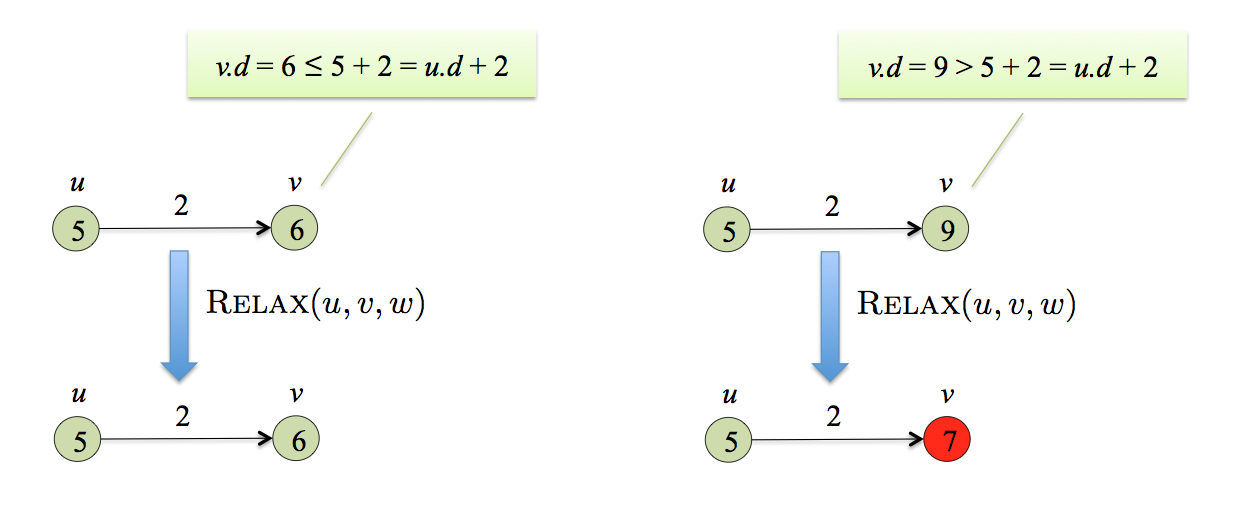
\includegraphics[scale = 0.6]{img01.png}
        \caption{Rilassamento di archi}
    \end{figure}
    
\subsection{Condizione di Bellman}
Per qualsiasi arco $(u,v) \in E$ si ha:
    \begin{equation}
        \delta(s, v) \leq \delta(s, u) + w (u, v)
    \end{equation}
    \begin{figure}[h!]
        \centering
        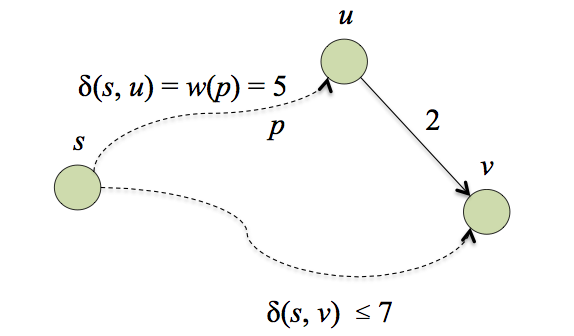
\includegraphics[scale = 0.7]{img02.png}
        \caption{Condizione di Bellman}
    \end{figure}
    
    
\subsection{Algoritmo di Dijkstra}
L'algoritmo di Dijkstra risolve il problema dei cammini minimi da sorgente unica in un grafo orientato pesato $G = (V, E)$ nel caso in cui tutti i pesi degli archi non siano negativi.\\
L'algoritmo di Dijkstra mantiene un insieme $S$ di vertici i cui pesi finali dei cammini minimi della sorgente $s$ sono stati già determinati. L'algoritmo seleziona ripetutamente il vertice $u \in (V-S)$ con la stima minima del cammino minimo, aggiunge $u \in S$ e rilassa tutti gli archi che escono da $u$.\\\\
Nella nostra implementazione manteniamo una coda di $min$-priorità $Q$ di vertici, utilizzando come chiavi i loro valori $d$.
    \begin{lstlisting}[caption = Algoritmo di Dijkstra]
        Dijkstra (G, w, s)
            Initialize-Single-Source (G, s)
            S = 0
            Q = G.V
            while (Q $\neq$ 0)
                u = Extract-Min(Q)
                S = S $\cup \{$ S $\}$
                for (each $v \in G.Adj[u]$)
                    Relax (u, v, w)
    \end{lstlisting}
